\cotefile{10}
\scanpage{131}

b) Exemple d'un $\otimes$ foncteur exact fidèle, compatible avec $\deleted{\unsure{k\handwritten{\varphi}|k\handwritten{\psi}|k\handwritten{\mu}}}$ $1,\handwritten{\unsure{\varphi|\phi|\psi}},{}^{\handwritten{\unsure{\vee|\nu|v}}}$ (mais pas \deleted{avec} $\handwritten{\unsure{\psi|\varphi|\mu}}$ !), et qui n'est pas localement isomorphe au foncteur fibre donné. - On prend pour $G$ un groupe. On note alors que la donnée d'un système de $\deleted{\unsure{M|W}}\handwritten{L}_{g}$ et d'isomorphismes $(\rlap{\(x\)}-)$ \deleted{, avec }\unsure{\deleted{$(\rlap{\(x\)}-\rlap{\(x\)}-)$}|$(\rlap{\(x\)}-\rlap{\(x\)}-)$}, satisfaisant les diverses compatibilités, est équivalente à la donnée d'une extension de $G$ par $k^{\handwritten{*}}$. Le foncteur $\inserted{F'}$ est isomorphe a\deleted{y}u foncteur $F$ sss cette extension splitte. L'ensemble des classes d'isomorphie de foncteurs fibres définis sur $k$ est ainsi en correspondance 1-1 avec $H^{2}(G,k^{\handwritten{*}})$. Or Même si $G$ est commutatif (pa\unsure{\deleted{f}r|\deleted{r}f} exemple le produit de deux groupes cycliques isomorphes d'ordre premier à \deleted{$k^{\handwritten{*}}$), et $k$} $\mathrm{car}.k$) et $k$ algébriquement clos, le $H^{2}$ peut être non nul; \deleted{il ne se tue alors dans} d'ailleurs un élément non nul de $H^{2}$ ne se tue dans aucune extension de $k$ (si $k$ alg. clos), d'après le principe de l'exten\deleted{i}s\deleted{o}i\deleted{n}on finie.

Si cependant $G$ est commutatif, et si on se borne aux $F'$ compatibles avec $\handwritten{\psi}$ également, on trouve les extensions commutatives de $G$ par $k^{\handwritten{*}}$; si $k$ est al\unsure{\deleted{e}g|g}\deleted{g}ébriquement clos, donc $k^{\handwritten{*}}$ divisible, alors toute telle extension splitte, donc $F'$ est alors isomorphe à $F$ (en conf\deleted{i}ormité avec la théorie galoisienne relative au cas où l'application diagonale de $U$ est commutative ...).

Ainsi, il peut y avoir des foncteurs fibres compatibles avec $\handwritten{\psi}$ donné, et d'autres qui ne le sont pas et qui par suite ne sont pas loc. isom. au premier. Cela montre donc \margin{\handwritten{étudier les contraintes de comm. \unsure{\&|+|\(\psi\)} \unsure{associer|associon|assoc.} aux graduations mod 2.}} qu'\deleted{i}o\deleted{l}n ne peut négliger la \deleted{condition de} contrainte de commutativité comme on aurait aimé pouvoir le faire. De plus, \margin{\handwritten{Exemple de foncteurs fibres gradués mod 2 non loc. isom. aux \unsure{vrais|sans} $\unsure{\deleted{\varphi}\uparrow\psi|(\uparrow\psi|\varphi\psi|\psi\varphi}$ ??}\figure{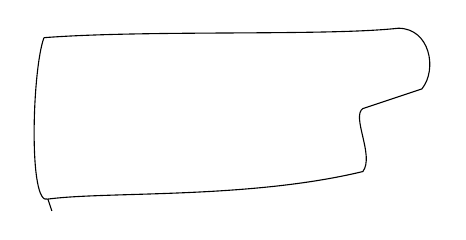
\begin{tikzpicture}[x=1cm,y=1cm]
\draw (0,0) .. controls (1.3,.1) and (3.6,.02) .. (4.5,.12) .. controls (4.9,.12) and (5,-.4) .. (4.8,-.65) -- (4.05,-.9) .. controls (3.9,-1) and (4.2,-1.5) .. (4.05,-1.7) .. controls (2.6,-2.05) and (.8,-1.95) .. (.05,-2.05) .. controls (-.2,-2.15) and (-.15,-.4) .. (0,0);
\draw (.05,-2.05)--(.1,-2.2);
\end{tikzpicture}}} cela suggère qu'en l'absence de contrainte de commutativité, la classification des foncteurs fibres se fait par des groupes du type de cohomologie de Brauer.

